\documentclass[10pt,letterpaper]{article}
\usepackage[top=0.85in,left=2.75in,footskip=0.75in]{geometry}
\setlength{\headheight}{43pt}

% Use adjustwidth environment to exceed column width (see example table in text)
\usepackage{changepage}

% Use Unicode characters when possible
\usepackage[utf8]{inputenc}

% textcomp package and marvosym package for additional characters
\usepackage{textcomp,marvosym}

% fixltx2e package for \textsubscript
\usepackage{fixltx2e}

% amsmath and amssymb packages, useful for mathematical formulas and symbols
\usepackage{amsmath,amssymb}

% cite package, to clean up citations in the main text. Do not remove.
\usepackage{cite}

% Use nameref to cite supporting information files (see Supporting Information section for more info)
\usepackage{nameref,hyperref}

% line numbers
\usepackage[right]{lineno}

% ligatures disabled
\usepackage{microtype}
\DisableLigatures[f]{encoding = *, family = * }

% rotating package for sideways tables
\usepackage{rotating}

% Remove comment for double spacing
%\usepackage{setspace} 
%\doublespacing

% Text layout
\raggedright
\setlength{\parindent}{0.5cm}
\textwidth 5.25in 
\textheight 8.75in

% Bold the 'Figure #' in the caption and separate it from the title/caption with a period
% Captions will be left justified
\usepackage[aboveskip=1pt,labelfont=bf,labelsep=period,justification=raggedright,singlelinecheck=off]{caption}

% Use the PLoS provided BiBTeX style
\bibliographystyle{plos2009}

% Remove brackets from numbering in List of References
\makeatletter
\renewcommand{\@biblabel}[1]{\quad#1.}
\makeatother

% Leave date blank
\date{}

% Header and Footer with logo
\usepackage{lastpage,fancyhdr,graphicx}
\pagestyle{myheadings}
\pagestyle{fancy}
\fancyhf{}
\lhead{
\includegraphics[natwidth=1.3in,natheight=0.4in]{PLOSlogo.png}}
\rfoot{\thepage/\pageref{LastPage}}
\renewcommand{\footrule}{\hrule height 2pt \vspace{2mm}}
\fancyheadoffset[L]{2.25in}
\fancyfootoffset[L]{2.25in}
\lfoot{\sf PLOS}

%% Include all macros below

\newcommand{\lorem}{{\bf LOREM}}
\newcommand{\ipsum}{{\bf IPSUM}}

%% END MACROS SECTION

\begin{document}
\vspace*{0.35in}

% Title must be 150 characters or less
\begin{flushleft}
{\Large
\textbf\newline{\textbf{Genomics Environments Characterization by means of Novel Fingerprints Features}}
}
\newline
% Insert Author names, affiliations and corresponding author email.
\\
Guillermo G. Torres\textsuperscript{1},
J. H. Martinez\textsuperscript{2,3}
\\
\bf{1} Biotechnology Institute, National University of Colombia, Bogotá D.C, Colombia
\\
\bf{2} Universidad del Rosario, Bogotá, Colombia
\bf{3} Technical University of Madrid, Madrid, Spain
\\

% Insert additional author notes using the symbols described below. Insert symbol callouts after author names as necessary.
% 
% Remove or comment out the author notes below if they aren't used.
%
% Primary Equal Contribution Note
%\Yinyang These authors contributed equally to this work.

% Additional Equal Contribution Note
%\ddag These authors also contributed equally to this work.

* E-mail: Corresponding ggtorrese@unal.edu.co
\end{flushleft}

% Please keep the abstract below 300 words
\section*{Abstract}
Bla bla bla

\linenumbers

\section*{Introduction}
The metatranscriptomics and metagenomics are new molecular approaches developed to explore the genetic potential of the ecosystems, bringing an unprecedented understanding of the relationships between microbial communities without the need of previews knowledge of them or their environment. This approaches allowed the first large-scale insight into the ecology of the environments since both taxonomical and functional diversity outlook.
	
Since an ecology perspective, a key step to characterize one ecosystem is studying its biodiversity, that implies to discover, to describe and to analyze the organization of all elements involved in, classifying both by evolutionary (phylogenetic) and ecological (functional) criteria \cite{Colwell:2009tr}. In this sense, a metagenomic and metatranscriptomic analysis is aiming to decipher the microbial community structure by characterizing some microbes residing therein and quantifying their diversity regarding some level of the biological population like species, genera, families, order or even patterns of evolutionary diversification and the richness as frequently employed diversity metric. Describing the number of distinct microbial taxa within a given unit area inhabiting a particular ecosystem, measured by the relative abundance, that refers to the quantity of rarity and commonness among taxonomical or functional individuals in the sample or community \cite{Colwell:2009tr,Mouillot:2004dq}.

Currently, high-throughput sequencing (HTS) technologies have offered the opportunity to obtain genomic and transcriptomic information at increasingly high throughput and low price. Consequently, studies aiming to investigate taxonomical and functional diversity use an approach referred to as shotgun sequencing, in which genomic or transcriptomic fragments originated from organisms constituting microbiome are extracted and massively sequenced \cite{Tyson:2004bw}. Habitually, the HTS technologies, the most commonly used Illumina and Roche454 platforms, generates millions of sequences, referred to as "reads", that could be considered to represent the compositional properties of their source genomes and transcripts. Subsequent analysis of the reads involves the process referred to as "binning". The reads derived from this mixture of different organisms are assigned to phylogenetic groups according to their taxonomic origins, analogous  to machine learning process, where the reads are clustered into distinct bins using reference sequences with known taxonomic origin like a supervised learning method.

In the binning process typically we attempt to classify the reads through two strategies: composition-based or similarity-based. The first involves comparison of information related to GC content \cite{Foerstner:2006uz}, codon usage \cite{Noguchi:2006tu} or K-mer frequency \cite{Sandberg:2001dw} from reads with those calculated from reference sequences. On the other hand, the similarity-based strategy uses string comparison algorithms between reads and reference sequences for data characterization. However, this last strategy can be sub-divided in two general methods: those to use Hidden Markov Models (HMM) \cite{Eddy:1998by} or BLAST-based homology searches \cite{Huson:2007jl,Haque:2009eh}.

Despite all efforts, the bioinformatic tools able to read binning are unable to make enough specific assignments for short fragments ($<$ 400pb)\cite{Brady:2009ia,Mende:2012bg}. Therefore, we present an enhancing of the HISS pipeline \cite{TorresEstupinan:2014dx}, an integrated approach that combines bioinformatic algorithms to fingerprint design and \textit{in silico} hybridization using BLAST algorithm to characterize the ecosystems assessing critical genes involved in a functional context.

% You may title this section "Methods" or "Models". 
% "Models" is not a valid title for PLoS ONE authors. However, PLoS ONE
% authors may use "Analysis" 
\section*{Materials and Methods}
Succeeding, we briefly describe the HISS pipeline and then present the algorithmic improvements implemented to fingerprint design and \textit{in silico} hybridization. The HISS pipeline consist of 2 main stages (Figure ~\ref{fig1}). The first phase is the fingerprint designer, this takes interest genes sequences and designs the best non-redundant fingerprints from each of them. Later, the hybridizer performs an \textit{in silico} hybridization between designed probes and the reads from metagenome or metatranscriptome, subsequently, the hybridization is evaluated.

\begin{figure}[!htpb] 
\caption{{\bf Overview of HISS pipeline stages.}
CrSo: Fingerprint designer. Hybridator: \textit{In silico} hybridization step.}
\centering
\label{fig1}
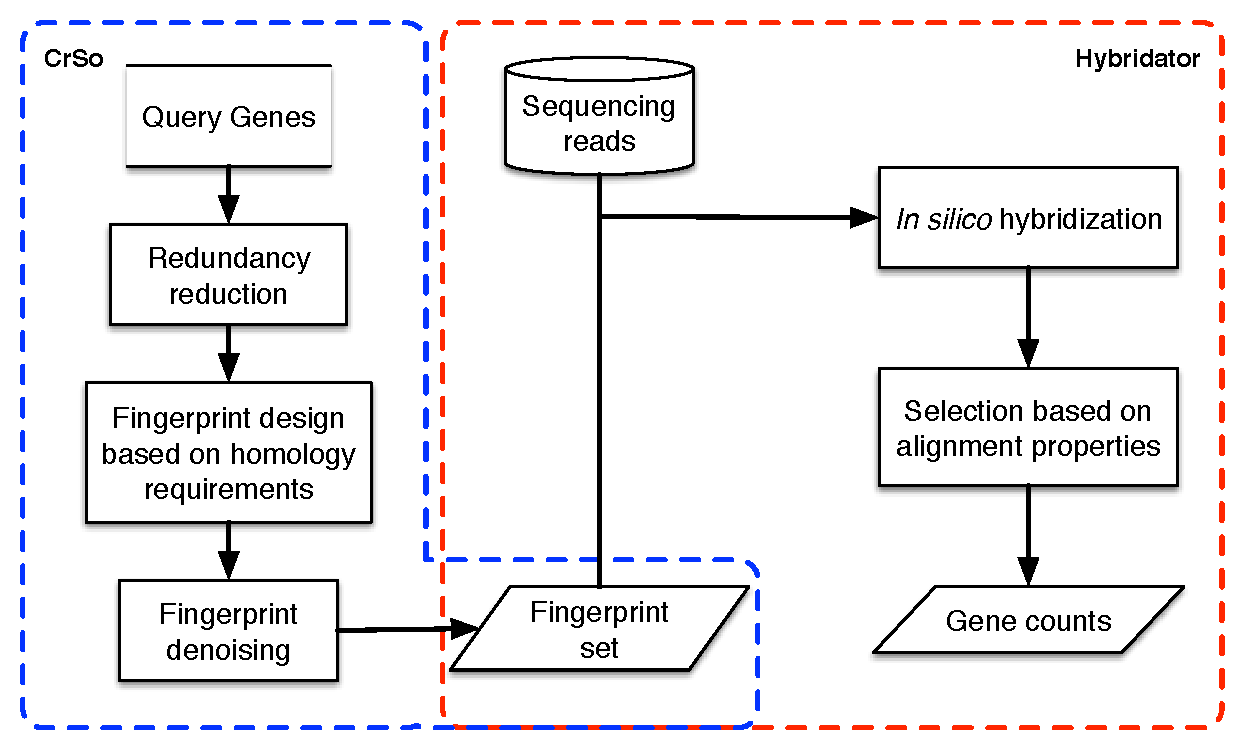
\includegraphics[width=0.8\textwidth,natwidth=610,natheight=642]{imgs/Fig1.pdf}\\

\end{figure}

\subsection*{Fingerprints design (CrSo).}

CrSo split up the fingerprint design in three general steps (Figure ~\ref{fig1}): 1) redundancy reduction 2) homology score calculation and best fingerprint compilation and 3) fingerprint denoising. At the first stage, CrSo performs a clusterization process using UCLUST \cite{Edgar:2010cv} program, at the end of this step several sequences that covering the same biological sequence, and sequence fragments of one biological sequence that are globally alignable will be eliminated from initial input data set.

For fingerprint metrics calculation, the previous version of CrSo used the program OligoWiz 2.0 \cite{Wernersson:2005ee}, however this software implement some algorithms to satisfy microarray experimental condition, such as melting temperature (T\textsubscript{m}) and GC content, not relevant by \textit{in silico} hybridization, therefore here we will focus on specificity constraint of the fingerprints. A fingerprint of given gene $g_t$ by definition will be any sub-sequence of gene $g_t$ that is not sub-sequence of any $g_i \in G, i \neq t$, where $G$ is a reference database of genes $G = \{g_1,g_2,g_3,...,g_N\}$ consisting of $N$ sequences. 

In order to prevent hybridization to unintended targets (cross-hybridization), CrSo estimates this cross-hybridization evaluating the similarity of the target gene with other transcripts using BLAST. CrSo calculates a homology score for each possible oligonucleotide (FIS), based on BLAST search of the taget gene against a reference database constituted by prokaryote, fungi and environmental sequences reported in EMBL-GeneBank-DDBJ \cite{Benson:2009fc} database. Each BLAST hit resulting is evaluated along the target sequence, where $M$ is the number of BLAST hits regarded by $j$ position of the target gene and $H = \{h_1j,...,h_Mj\}$ be the BLAST hits identity in position $j$.



(Figure ~\ref{fig2}).

 the homology score for the probes the fingerprint was consider a sub-string of the genes, where they were a strigs with 

  

\begin{figure}[!htpb] 
\caption{{\bf Overview of CrSo pipeline.}
%CrSo: Fingerprint designer. Hibridator: \textit{In silico} hibridization step.
}
\centering
\label{fig2}
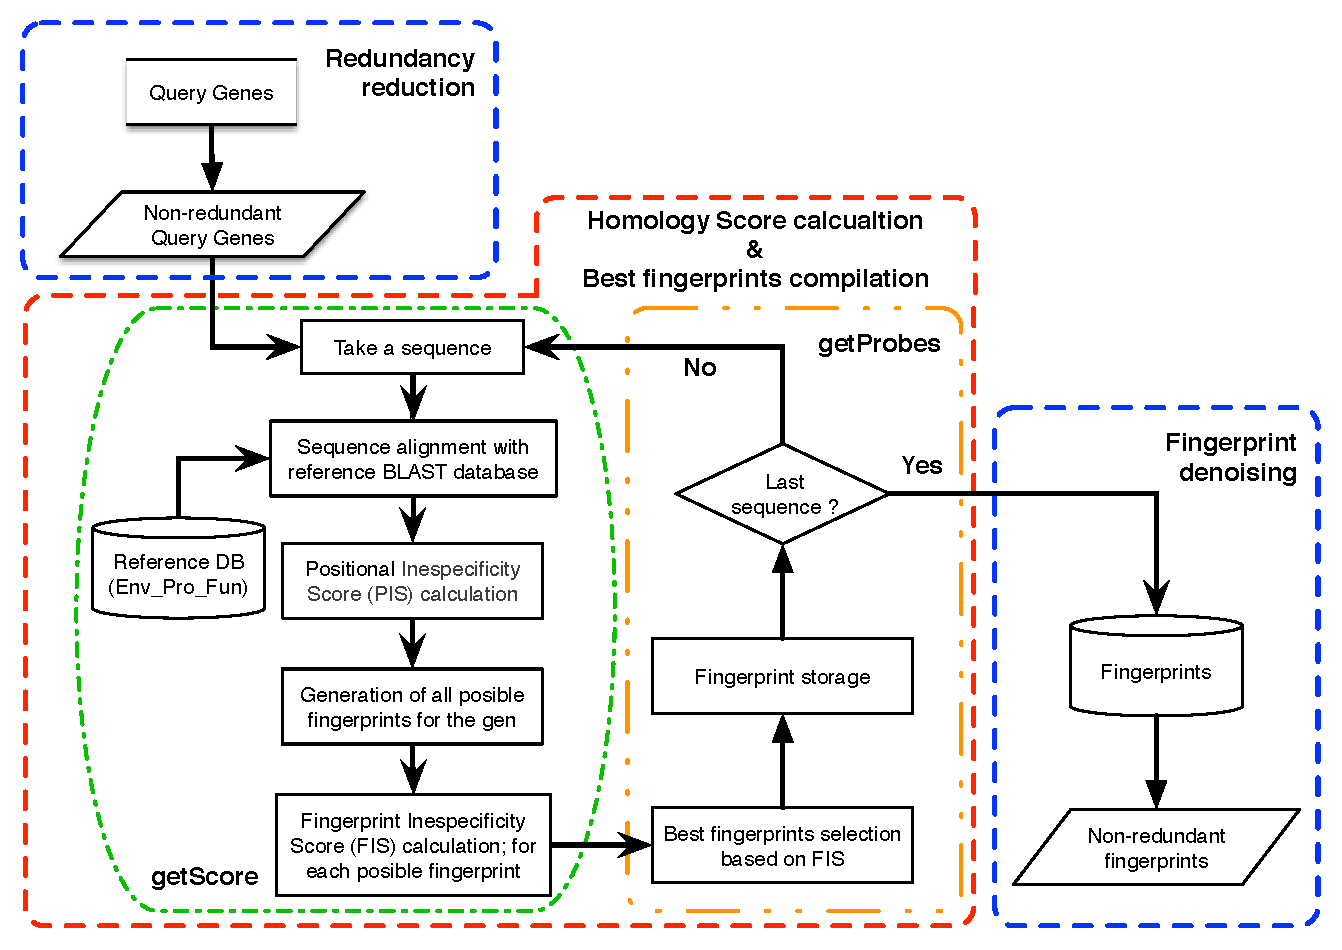
\includegraphics[width=1\textwidth,natwidth=610,natheight=642]{imgs/Fig2.pdf}\\

\end{figure}


In the second stage, HISS uses the fingerprints designed to make an \textit{in silico} hibridization with the reads from metagenomic or metatrasncriptomic sample following a general rule: each read aligned significantly with a fingerprint should be considered originated or homologous of the enzyme gene that fingerprint represents.

\begin{equation}\label{eq:schemeP}
D_{coll} = \frac{D_f+\frac{[S]^2}{K_D S_T} D_S} {1+\frac{[S]^2}{K_D S_T}},
D_{sm} = \frac{D_f+ \frac{[S]}{K_D} D_S}{1+\frac{[S]}{K_D}},
\end{equation}


\begin{figure}[!htpb]
\caption{{\bf Figure Title first bold}
Figure  A: Lorem. B: Consectetur.}
\label{fig3}
\end{figure}

\subsection*{\textit{In Silico} Hibridization}

\begin{enumerate}
\item{react}
\item{diffuse free particles}
\item{increment time by dt and go to 1}
\end{enumerate}

% Results and Discussion can be combined.
\section*{Results}
Nulla Table~\ref{table1} volutpat.

\begin{table}[!ht]
\begin{adjustwidth}{-2.25in}{0in} % Comment out/remove adjustwidth environment if table fits in text column.
\caption{
{\bf Table caption title.}}
\begin{tabular}{|l|l|l|l|l|l|l|l|}
\hline
\multicolumn{4}{|l|}{\bf Heading1} & \multicolumn{4}{|l|}{\bf Heading2}\\ \hline
$cell1 row1$ & cell2 row 1 & cell3 row 1 & cell4 row 1 & cell5 row 1 & cell6 row 1 & cell7 row 1 & cell8 row 1\\ \hline
$cell1 row2$ & cell2 row 2 & cell3 row 2 & cell4 row 2 & cell5 row 2 & cell6 row 2 & cell7 row 2 & cell8 row 2\\ \hline
$cell1 row3$ & cell2 row 3 & cell3 row 3 & cell4 row 3 & cell5 row 3 & cell6 row 3 & cell7 row 3 & cell8 row 3\\ \hline
\end{tabular}
\begin{flushleft} Table notes.
\end{flushleft}
\label{table1}
\end{adjustwidth}
\end{table}


\subsection*{Probe Design.}

Maecenas.

\subsection*{Annotation.}

Nulla
% Please do not create a heading level below \subsection. For 3rd level headings, use \paragraph{}.
\paragraph{Taxonomical annotation} Nulla.
\paragraph{Functional annotation} Nulla.

\section*{Discussion}
Nulla Table~\ref{table1} volutpat. 

\subsection*{\lorem\ and \ipsum\ Nunc.}

CO\textsubscript{2} Maecenas. For more information, see \nameref{S1_Text}.

\section*{Supporting Information}

% Include only the SI item label in the subsection heading. Use the \nameref{label} command to cite SI items in the text.
\subsection*{S1 Video}
\label{S1_Video}
{\bf Bold the first sentence.}  Maecenas.

\subsection*{S1 Text}
\label{S1_Text}
{\bf Lorem Ipsum.} Maecenas.

\subsection*{S1 Fig}
\label{S1_Fig}
{\bf Lorem Ipsum.} Maecenas.

\subsection*{S1 Table}
\label{S1_Table}
{\bf Lorem Ipsum.} Maecenas.

% Do NOT remove this, even if you are not including acknowledgments.
\section*{Acknowledgments}
Cras.

\nolinenumbers

%\section*{References}
% Either type in your references using
% \begin{thebibliography}{}
% \bibitem{}
% Text
% \end{thebibliography}
%
% OR
%
% Compile your BiBTeX database using our plos2009.bst
% style file and paste the contents of your .bbl file
% here.
% 

\begin{thebibliography}{10}
\bibitem{Colwell:2009tr}
Colwell, R. K. (2009). Biodiversity: concepts, patterns, and measurement. The Princeton Guide to Ecology.

\bibitem{Mouillot:2004dq}
Mouillot, D., Mason, W. H. N., Dumay, O., Wilson, J. B. (2004). Functional regularity: a neglected aspect of functional diversity. Oecologia, 142(3), 353–359. doi:10.1007/s00442-004-1744-7

\bibitem{Tyson:2004bw}
Tyson, G. W., Chapman, J., Hugenholtz, P., Allen, E. E., Ram, R. J., Richardson, P. M., et al. (2004). Community structure and metabolism through reconstruction of microbial genomes from the environment. Nature, 428(6978), 37–43. doi:10.1038/nature02340

\bibitem{Foerstner:2006uz}
Foerstner, K. U., Mering, von, C., Bork, P. (2006). Comparative Analysis of Environmental Sequences: Potential and Challenges. Philosophical Transactions: Biological Sciences, 361(1467), 519–523.

\bibitem{Noguchi:2006tu}
Noguchi, H., Park, J., Takagi, T. (2006). MetaGene: prokaryotic gene finding from environmental genome shotgun sequences. Nucleic Acids Res.

\bibitem{Sandberg:2001dw}
Sandberg, R. R., Winberg, G. G., Bränden, C. I. C., Kaske, A. A., Ernberg, I. I., Cöster, J. J. (2001). Capturing whole-genome characteristics in short sequences using a naïve Bayesian classifier. Genes \& Development, 11(8), 1404–1409. doi:10.1101/gr.186401

\bibitem{Eddy:1998by}
Eddy, S. R. (1998). Profile hidden Markov models. Bioinformatics (Oxford, England), 14(9), 755–763. doi:10.1093/bioinformatics/14.9.755

\bibitem{Huson:2007jl}
Huson, D. H., Auch, A. F., Qi, J., Schuster, S. C. (2007). MEGAN analysis of metagenomic data. Genome Research, 17(3), 377–386. doi:10.1101/gr.5969107

\bibitem{Haque:2009eh}
Haque, M., Ghosh, T. S., Komanduri, D., Mande, S. S. (2009). SOrt-ITEMS: Sequence orthology based approach for improved taxonomic estimation of metagenomic sequences. Bioinformatics (Oxford, England), 25(14), 1722–1730. doi:10.1093/bioinformatics/btp317

\bibitem{Brady:2009ia}
Brady, A., \& Salzberg, S. L. (2009). Phymm and PhymmBL: metagenomic phylogenetic classification with interpolated Markov models. Nature Methods, 6(9), 673–676. doi:10.1038/nmeth.1358

\bibitem{Mende:2012bg}
Mende, D. R., Waller, A. S., Sunagawa, S., Järvelin, A. I., Chan, M. M., Arumugam, M., et al. (2012). Assessment of metagenomic assembly using simulated next generation sequencing data. PloS One, 7(2), e31386. doi:10.1371/journal.pone.0031386

\bibitem{TorresEstupinan:2014dx}
Torres-Estupiñan, G. G., Barreto-Hernández, E. (2014). In Silico Hybridization System for Mapping Functional Genes of Soil Microorganism Using Next Generation Sequencing. In Advances in Computational Biology (Vol. 232, pp. 337–344). Cham: Springer International Publishing. doi:10.1007/978-3-319-01568-2\_48

\bibitem{Edgar:2010cv} 
Edgar, R. C. (2010). Search and clustering orders of magnitude faster than BLAST. Bioinformatics (Oxford, England), 26(19), 2460–2461. doi:10.1093/bioinformatics/btq461

\bibitem{Wernersson:2005ee}
Wernersson, R., Nielsen, H. B. (2005). OligoWiz 2.0--integrating sequence feature annotation into the design of microarray probes. Nucleic Acids Research, 33(Web Server issue), W611–5. doi:10.1093/nar/gki399

\bibitem{Benson:2009fc}
Benson, D. A., Karsch-Mizrachi, I., Lipman, D. J., Ostell, J., \& Sayers, E. W. (2009). GenBank. Nucleic Acids Research, 38(Database), D46–D51. doi:10.1093/nar/gkp1024


\end{thebibliography}

\end{document}

